\subsection{Original target and checkpoint comparisons}
At 80\% coverage, validation-selected seven-output Swin-T has mean complete-vote disagreement of 23.68\% for Soft and 24.06\% for Uniform (Table~\ref{tab:primary}). Soft minus Uniform is -0.38 percentage points (pp), with a conditional 95\% pixel-cluster interval of [-0.64, -0.07]. Each model accepts its own 2,620 images. The corresponding Soft-minus-Hard difference is -2.61 pp [-2.98, -2.19]; the substantially smaller matched-control difference changes the interpretation of that hard--soft comparison.
\begin{table}[!htbp]
\caption{Selected-checkpoint risk at 80\% coverage (2,620 of 3,275 images). Risk is mean $\pm$ sample SD; components are mean percentage points}\label{tab:primary}
\centering\begin{tabular}{lrrrr}\toprule
Targets & Risk (\%) & Unsupported & Ambiguity & Excess\\\midrule
Hard & $26.30 \pm 1.04$ & 6.65 & 16.14 & 3.51\\
Tie-hard & $25.82 \pm 0.58$ & 6.67 & 16.03 & 3.13\\
Uniform & $24.06 \pm 0.10$ & 6.41 & 15.41 & 2.24\\
Tie-Uniform & $24.27 \pm 0.17$ & 6.47 & 15.46 & 2.35\\
Soft & $23.68 \pm 0.07$ & 6.55 & 15.01 & 2.13\\
\bottomrule\end{tabular}\par
Accepted identities differ; components provide accounting, not causal attribution.
\end{table}


Tie-hard minus Hard is -0.47 pp [-0.80, -0.12], and Soft minus Tie-hard is -2.14 pp [-2.49, -1.76]. At fixed epoch 12, Soft minus Uniform remains negative (-0.32 pp [-0.63, -0.05]), whereas Soft minus Hard is -1.35 pp [-1.72, -1.05]. Soft also has lower disagreement than Tie-Uniform at both Swin checkpoint states. The supplement retains all seed differences, absolute risks, selected epochs, trajectories and coverage curves; these are correlated sensitivities on the same image source, not additional independent confirmations.

\subsection{Distributional agreement and backbone sensitivity}\label{sec:distance}
Soft has lower ten-category squared distance than Uniform and Tie-Uniform in every original seed, backbone and checkpoint state. For selected Swin-T, the means are 0.09783 versus 0.11571 and 0.11373 (Table~\ref{tab:distance}). This scores all 3,275 primary-test images, without rejection.
\begin{table}[!htbp]
\caption{Complete-vocabulary squared distances: means across three seeds on all 3,275 primary-test images. Values are unscaled distance units; lower is better}\label{tab:distance}
\centering\small\begin{tabular}{llrrr}\toprule
Backbone & State & Soft & Uniform & Tie-Uniform\\\midrule
Swin-T & Selected & 0.09783 & 0.11571 & 0.11373\\
Swin-T & Epoch 12 & 0.09779 & 0.11699 & 0.11280\\
ResNet-18 & Selected & 0.11059 & 0.12303 & 0.11805\\
ResNet-18 & Epoch 12 & 0.11089 & 0.12259 & 0.11665\\
\bottomrule\end{tabular}
\end{table}

The selective result is less consistent. Selected ResNet-18 gives Soft minus Uniform of +0.173 pp, compared with -0.378 pp for Swin-T; all four ResNet conditional intervals cross zero. Figure~\ref{fig:backbones} displays both outcomes with their distinct scales. Fixed-epoch values and all per-seed distributional scores appear in Supplementary Sect.~S2. These findings establish a difference between the measured outcomes for the tested models, without establishing a general architecture ordering.
\begin{figure}[!htbp]
\centering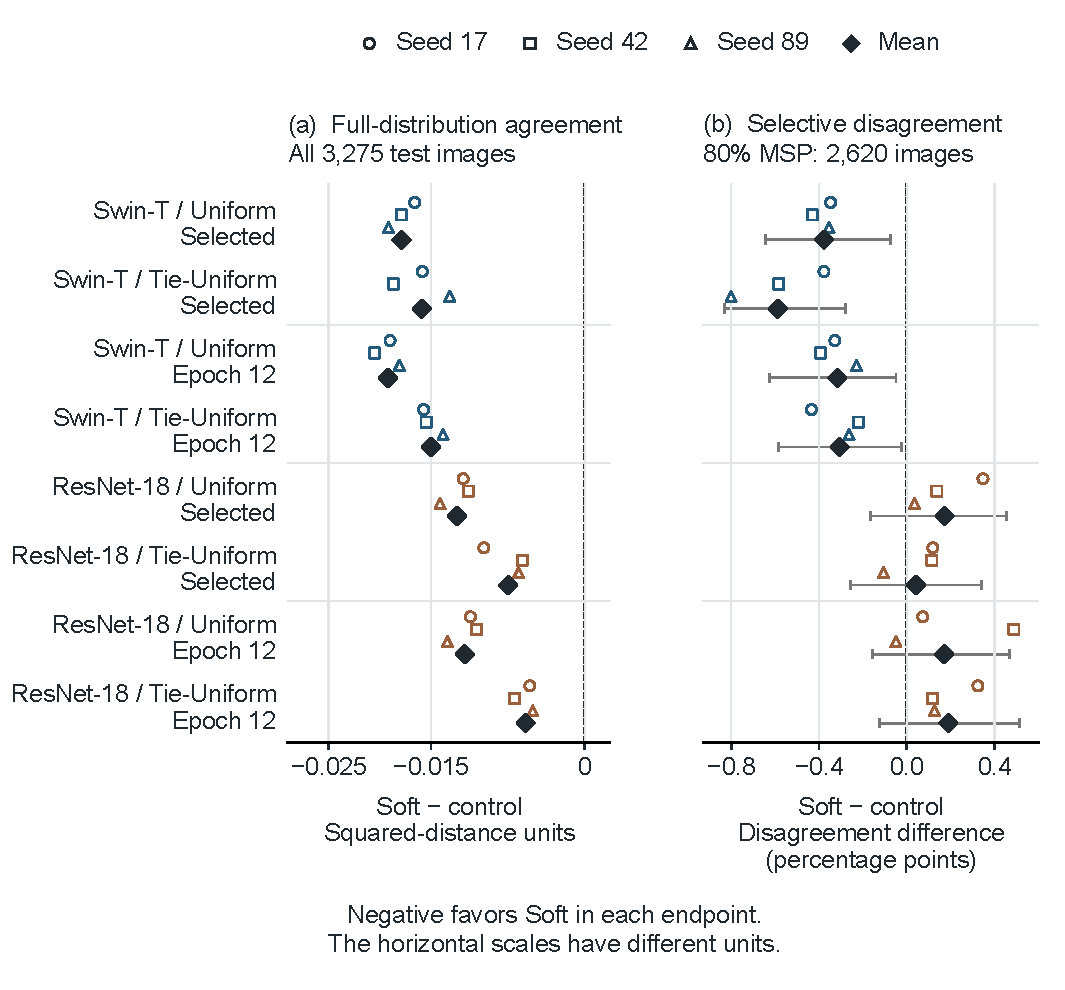
\includegraphics[width=\linewidth]{final_revision_2026_10_20/source/figures/Fig7.pdf}
\caption{Original Soft-minus-control differences. (a) Squared distance on all 3,275 images. (b) Complete-vote disagreement at 80\% own-ranking coverage. Symbols show three paired-seed contrasts and their mean; bars in (b) are conditional 95\% pixel-cluster intervals. No interval is shown in (a). The panels have different units and scales. Negative favors Soft}\label{fig:backbones}
\end{figure}

\subsection{Minority allocation and the eight-expression follow-up}\label{sec:new-results}
Preserving target probability values does not preserve the selective result. Distance-selected seven-output Soft has mean disagreement of 23.68\%, compared with 24.48\% for Permutation: a difference of $-0.794$ pp, with a conditional 95\% interval of $[-1.071,-0.474]$. The three paired differences are $-0.523$, $-0.935$ and $-0.924$ pp (sample SD 0.235 pp). At epoch 12, the mean remains negative ($-0.548$ pp, interval $[-0.855,-0.261]$). Thus, the observed minority allocation performs better than this particular entropy- and maximum-preserving permutation. The control changes aggregate class priors, so the comparison does not uniquely isolate category identity from those priors.

The principal eight-output comparison gives Soft 23.74\% disagreement, Uniform 24.58\% and Tie-Uniform 23.79\%. Soft minus Uniform is $-0.836$ pp, interval $[-1.152,-0.509]$, with paired differences $-0.454$, $-1.191$ and $-0.863$ pp (SD 0.369 pp). This contrast remains negative at epoch 12 ($-0.385$ pp) and under risk-based checkpoint selection ($-0.585$ pp). In contrast, Soft minus Tie-Uniform is only $-0.052$ pp, interval $[-0.314,+0.212]$. Its epoch-12 and risk-selected means are $-0.130$ and $-0.104$ pp, respectively; both intervals also cross zero. These intervals do not establish equivalence. Figure~\ref{fig:followup-contrasts} retains all eight planned contrasts, rather than only the larger differences against Uniform.

\begin{figure}[!htbp]
\centering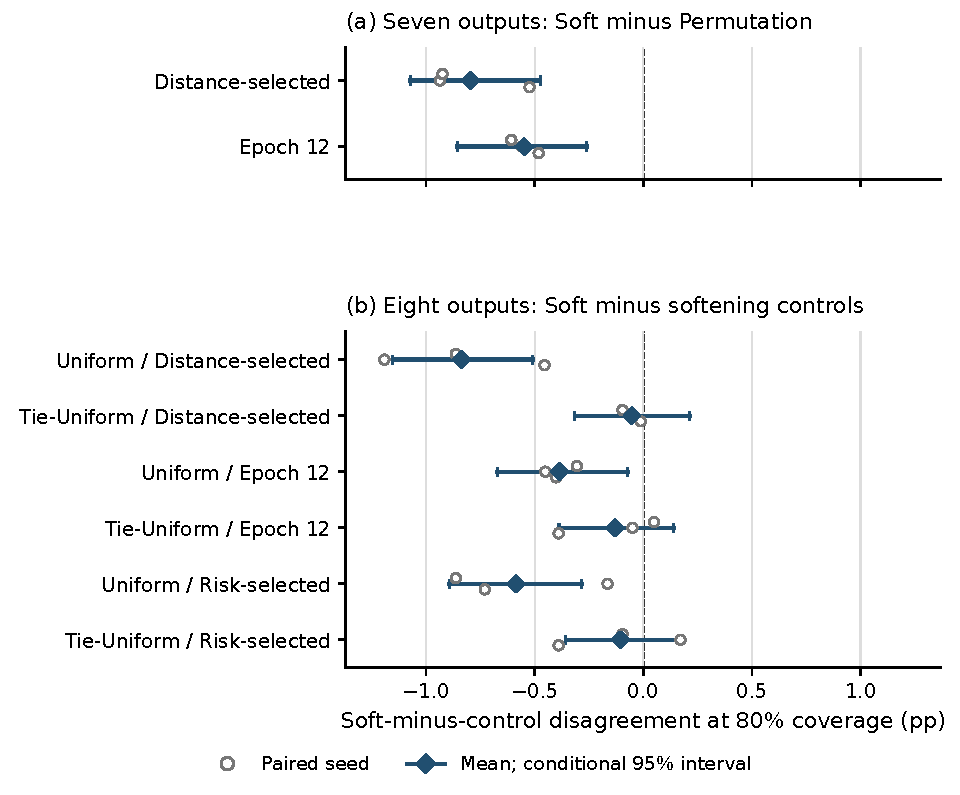
\includegraphics[width=\linewidth]{final_revision_2026_10_20/source/figures/FollowupContrasts.pdf}
\caption{Final adaptive follow-up at 80\% own-MSP coverage. Hollow symbols show three paired-seed differences, diamonds their mean, and bars conditional 95\% exact-pixel-cluster intervals. (a) Seven-output Soft minus Permutation. (b) Eight-output Soft minus Uniform or Tie-Uniform under all three checkpoint rules. Negative favors Soft. Distance selection is the principal rule; fixed epoch and risk selection are sensitivities. Different rules can select the same weights, and intervals do not represent uncertainty over new training seeds}\label{fig:followup-contrasts}
\end{figure}

Full-coverage distributional agreement remains more consistent. Eight-output Soft has lower ten-category squared distance than both softening controls in every seed and checkpoint rule. Distance-selected means are 0.09467 for Soft, 0.11708 for Uniform and 0.10962 for Tie-Uniform. However, expanding the vocabulary does not by itself establish a selective improvement: the seven- and eight-output Soft means are 23.68\% and 23.74\% on their separately accepted sets. This policy comparison changes supported weights, classifier dimension and fitted predictions together.

The new fixed-image comparisons also distinguish predictor changes from selection changes. For distance-selected eight-output models, Soft minus Uniform is $-0.729$ pp on Soft's accepted images and $-0.132$ pp on Uniform's images. Soft minus Tie-Uniform changes sign: $-0.279$ pp on Soft's images and $+0.125$ pp on Tie-Uniform's. The corresponding seven-output Soft-minus-Permutation means are $-0.523$ pp on Soft's set and $-0.074$ pp on Permutation's. These are means on identical images within each selector, not a causal decomposition of the own-ranking differences.

The separately frozen ranking extension reinforces the distinction. Calibration chose MSP over centered normalization for every new state, as it had for the original 48 states. For distance-selected eight-output Soft minus Tie-Uniform, the mean changes from $-0.052$ pp with MSP to $+0.280$ with margin, $+0.164$ with negative entropy and $+0.131$ with centered normalization. Predictions are unchanged; the accepted images change. Soft minus Uniform remains negative under these distance-selected scores, but its epoch-12 margin contrast is approximately zero ($+0.003$ pp). Supplementary Sect.~S11 retains every new state, seed, selected epoch, fixed-image comparison and ranking sensitivity. The findings support a conditional benefit against specific controls, not a score-independent advantage from retaining the full vote distribution.


\subsection{Identical images and annotation references}
Selected Swin-T's predictor ordering depends on who selects the images: Soft minus Uniform is +0.085 pp on Uniform-selected images but -0.352 pp on Soft-selected images (Fig.~\ref{fig:cross}). Within each set, the annotation reference and images are fixed, so the comparison concerns category choices. Changing from Uniform's set to Soft's set gives -0.025 pp for a fixed Uniform predictor and -0.463 pp for a fixed Soft predictor; mean Jaccard overlap is 0.8408. ResNet likewise changes sign between Uniform-selected (+0.445 pp) and Soft-selected images (-0.412 pp). The supplement retains both states and all seed matrices.
\begin{figure}[!htbp]
\centering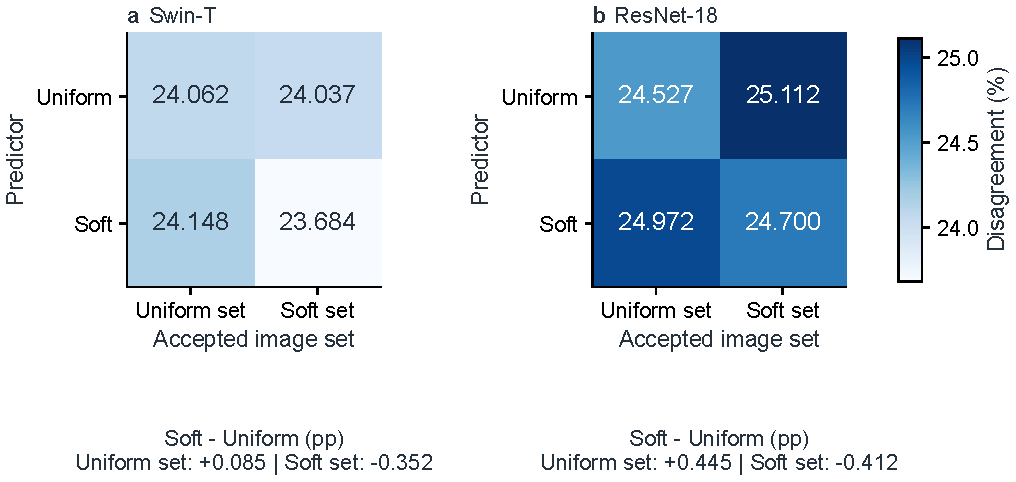
\includegraphics[width=\linewidth]{final_revision_2026_10_20/source/figures/Fig4.pdf}
\caption{Fixed-image cross-evaluation at 80\% coverage for selected (a) Swin-T and (b) ResNet-18. Cells show mean complete-vote disagreement (\%) across three seeds. Columns fix the selector's 2,620-image set; rows change the predictor. Signed Soft-minus-Uniform differences therefore hold images fixed. Each model's own-set risk uses different images}\label{fig:cross}
\end{figure}

The categorical reference also changes measured performance. On the same 2,484 supported-majority images, selected Swin-T Soft has weighted F1 0.6685 against original FER2013 labels and 0.9270 against crowd-majority labels. Against original labels, its score is 0.5722 on the full 3,275-image population. The first comparison changes the reference; the second changes the images. Neither changes the model predictions or establishes a new benchmark accuracy. Supplementary Sect.~S3 supplies complete same-image scores and the reference correspondence matrix.

\subsection{Unsupported categories and calibration transfer}
The original primary test set contains 1,732 fully supported, 1,527 partly supported and 16 zero-supported-mass images. At separately ranked 80\% within-stratum coverage, Soft/Uniform disagreement is 10.42\%/10.94\% for fully supported images and 40.00\%/40.58\% for partly supported images. The overall contrast is therefore not confined to images receiving unsupported votes. However, Soft accepts a mean 11.00 of the 16 zero-mass images, versus 7.00 for Uniform and 6.67 for Tie-Uniform. Lower overall disagreement does not imply better rejection of those inputs. Supplementary Sect.~S4 gives the global and within-stratum results, with contempt, unknown and not-a-face reported separately.

Empirical calibration fails to preserve its nominal targets: all 36 nonempty original test settings exceed them. These overlapping settings are not independent trials. At the 10\% target, Soft achieves 49.54\% coverage and 13.01\% risk, versus Hard's 38.35\% and 11.45\%. This is not an equal-achieved-risk coverage advantage.

The full-population annotation floor rises from 23.70\% in calibration to 26.67\% in testing, while unsupported mass rises from 5.72\% to 7.88\%. On Soft's accepted sets at the 20\% target, the +2.57 pp risk gap comprises +1.98 pp unsupported mass, +0.78 pp supported ambiguity and -0.19 pp excess (Fig.~\ref{fig:transfer}). These quantities describe rather than cause the gap. Calibration half-split holdout-minus-fit gaps average +0.05 to +0.19 pp, with broad descriptive 5th--95th-percentile ranges around -2.3 to +2.8 pp. The fixed-grid comparator yields 24 nonempty test settings with no overshoot, but fully abstains at the 10\% target for every condition and seed. Supplementary Sect.~S6 retains all thresholds, resamples and achieved risks.
\begin{figure}[!htbp]
\centering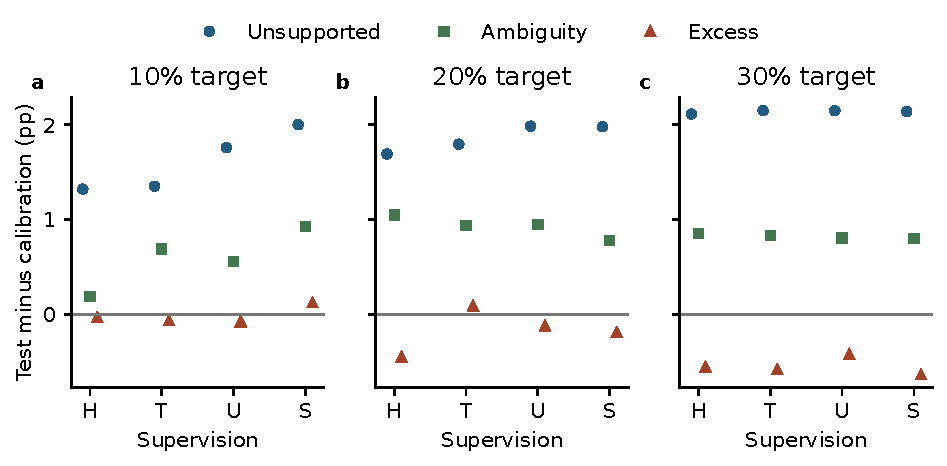
\includegraphics[width=\linewidth]{final_revision_2026_10_20/source/figures/Fig6.pdf}
\caption{Original calibration-to-test risk accounting. Mean differences in unsupported mass, supported ambiguity and excess sum to the risk gap on the respective accepted sets. H: Hard; T: Tie-hard; U: Uniform; S: Soft. Panels share a scale. These are descriptive components, not identified causes}\label{fig:transfer}
\end{figure}

\subsection{External clip transfer}
All 1,440 clips and 11,520 sampled frames meet the frozen rules, giving 100\% maximum coverage. At 80\% own-MSP coverage, selected Swin-T Soft has raw-reference disagreement of 68.37\%, Uniform 67.75\% and Tie-Uniform 67.42\%. Merging calm into neutral changes these to 60.72\%, 60.62\% and 60.03\%, while scoring the same predictions and accepted clips. This is agreement with human responses, not intended-expression accuracy.

The selected Swin Soft-minus-Uniform contrasts are -0.052, +2.639 and -0.755 pp for seeds 17, 42 and 89 under raw scoring: mean +0.611 pp, conditional actor interval [+0.23, +1.09]. Merged scoring gives -1.276, +2.483 and -0.903 pp: mean +0.101 pp [-0.26, +0.59]. Contrasts use unrounded risks. The positive mean is driven by seed 42 and does not establish a stable ordering over retraining. All three epoch-12 Swin contrasts favor Soft under merged scoring, illustrating checkpoint dependence. Figure~\ref{fig:external} and Supplementary Sect.~S7 retain both controls, backbones, states and references.
\begin{figure}[!htbp]
\centering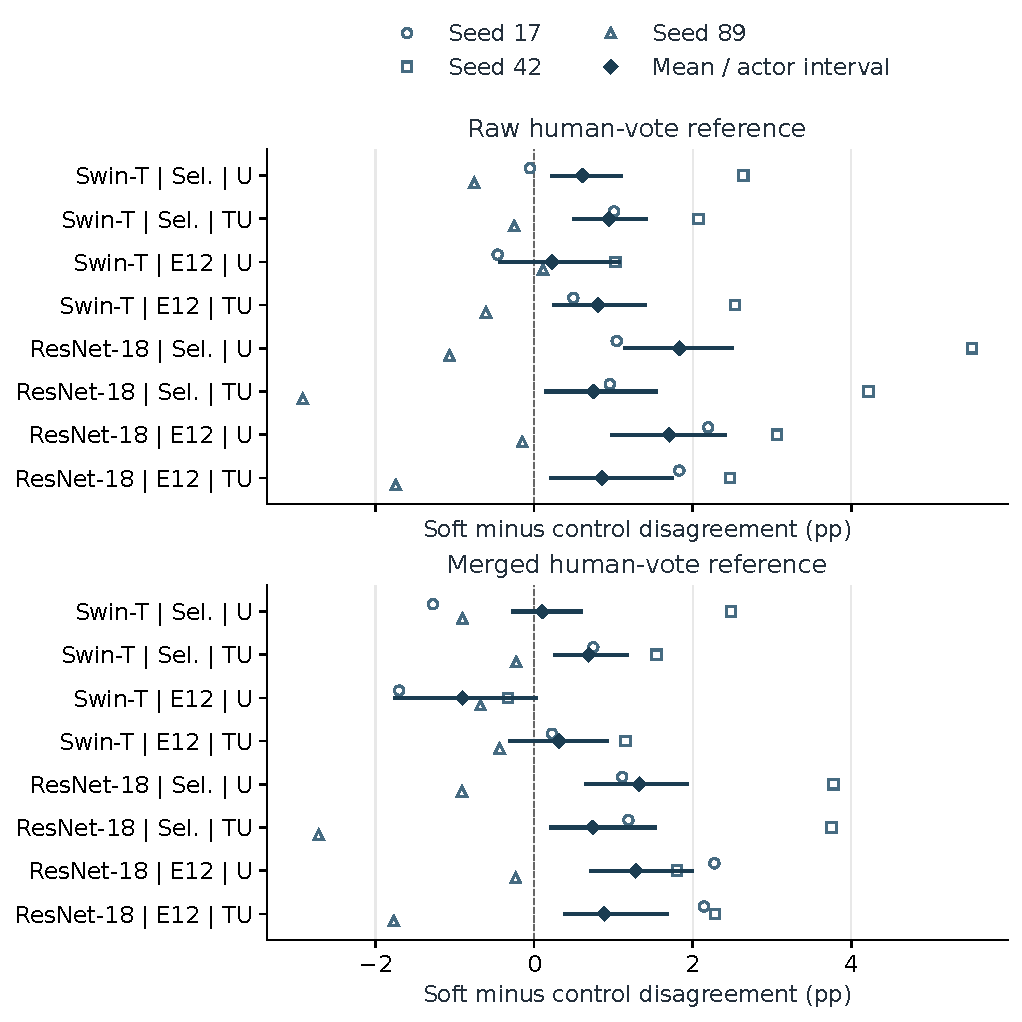
\includegraphics[width=\linewidth]{final_revision_2026_10_20/source/figures/ExternalContrasts.pdf}
\caption{Original external Soft-minus-control disagreement differences at 80\% own-MSP coverage. Hollow symbols show paired seeds; diamonds and bars show means and conditional 95\% actor-cluster intervals. Sel.: distance-selected; E12: epoch 12; U: Uniform; TU: Tie-Uniform. Negative favors Soft. The shared scale exposes seed variation; intervals condition on fitted pairs and observed actors/votes, not new seeds or raters}\label{fig:external}
\end{figure}

Transfer is poor for all conditions. Selected Swin Soft's raw all-clip risk is 71.06\%, comprising 11.90 pp unsupported mass, 16.81 pp supported ambiguity and 42.36 pp excess. On its accepted set, risk is 68.37\%, comprising 14.00, 16.61 and 37.76 pp, respectively. Thus, missing output categories alone cannot account for failure. Neutral comprises 67.0--70.0\% of accepted Soft predictions and 62.7--68.3\% of Uniform predictions. Vote-weighted matrices and eight-bin summaries describe these outputs, without treating clip labels as frame accuracy or assigning a cause to capture, population or aggregation. The follow-up aggregation and constant-category references below examine part of this interpretive uncertainty.
